\section{Results and Discussion}
\label{sec:results_discussion}

\newcommand{\fillertext}{Lorem ipsum dolor sit amet, consectetur adipiscing elit, sed do eiusmod tempor incididunt ut labore et dolore magna aliqua. Ut enim ad minim veniam, quis nostrud exercitation ullamco laboris nisi ut aliquip ex ea commodo consequat. Duis aute irure dolor in reprehenderit in voluptate velit esse cillum dolore eu fugiat nulla pariatur. Excepteur sint occaecat cupidatat non proident, sunt in culpa qui officia deserunt mollit anim id est laborum.}
\newcommand{\placeholderpar}[1]{{\color{gray}\textit{[Placeholder: #1]} \fillertext\par}}

\subsection{Overall segmentation performance}
\label{subsec:results_overall}

Table~\ref{tab:global_baseline} reports Dice and the centerline recall $R_{\mathrm{cl}}$ and precision $P_{\mathrm{cl}}$ of the five models over vessels of every radius. Here, and in every comparison across architectures below, the CNNs were trained from scratch and the transformer-based models were fine-tuned from their pre-trained weights. The best model of each retinal dataset reached a Dice close to published values: 82.3\% on DRIVE (\litemedsam{}) and 81.7\% on HRF (\medsam{}), against 82.8 and 81.0\% reported for Little W-Net~\cite{galdran2020littlewnetcouldstateoftheart}, and 92.2\% on FIVES (\medsam{}), against 90.4\% reported for FR-UNet~\cite{liu2022frunet} by Fadugba et al.~\cite{fadugba2024benchmarking}. VessMap has no published Dice to compare with. \lwnet{}, our implementation of Little W-Net, stayed 1.7 to 4.1 points below the published values: those of Little W-Net on DRIVE and HRF and the 85.7\% reported for W-Net on FIVES~\cite{fadugba2024benchmarking}. The published protocols differ from ours in the threshold, the evaluated pixels, the HRF training set and the loss (Appendix~\ref{app:results_detail}). Our training protocol aimed at the same training conditions for every model, not at the best published setup of each model, so we accept this difference and did not investigate it further.

No model had the highest mean on every dataset and metric, but in Dice a transformer-based model had the highest mean on every dataset: \litemedsam{} on DRIVE and \medsam{} on HRF and FIVES were significantly higher than every CNN. On VessMap, only \convnext{} was significantly lower than the other models. \convunext{}'s mean Dice on DRIVE is lowered by one test image on which it failed (Dice 14.5\%), so it was not significantly different from \lwnet{} or \medsam{}, although their means are higher.

Except for the centerline metrics on DRIVE, these overall metrics say little about thin vessels. $R_{\mathrm{cl}}$ and $P_{\mathrm{cl}}$ weigh every centerline pixel equally, and thin vessels hold 55.3\% of the ground-truth centerline pixels of DRIVE but 2.3 to 11.7\% of those of the other three datasets (computed from the pixel counts of Fig.~\ref{fig:recall_caliber}). Dice counts vessel pixels, so a wide vessel weighs more than a thin vessel of the same length. Fig.~\ref{fig:recall_caliber} therefore splits the centerline recall by vessel radius.

\subsection{Thin vessels: the plain ViT against the CNNs}
\label{subsec:results_thin}

Centerline recall fell as the vessel radius decreased, for every model (Fig.~\ref{fig:recall_caliber}). The first bin, radius below 1.5~px, had the lowest value in all 20 model--dataset pairs; this value is the centerline recall of thin vessels, $\thinrecall$, compared below.

Fine-tuned \medsam{} had an $\thinrecall$ within or above the range of the three CNNs, that is, between their lowest and highest means or above them, on every dataset. It was not significantly different from that of the best CNN, the CNN with the highest mean for that dataset and metric, on any dataset (Table~\ref{tab:medsam_vs_cnn}), and it was not significantly lower than that of any CNN. The hybrid \litemedsam{} had the highest mean $\thinrecall$ on every dataset, significantly above every CNN on DRIVE and HRF.

\begin{figure*}[tbp]
\centering
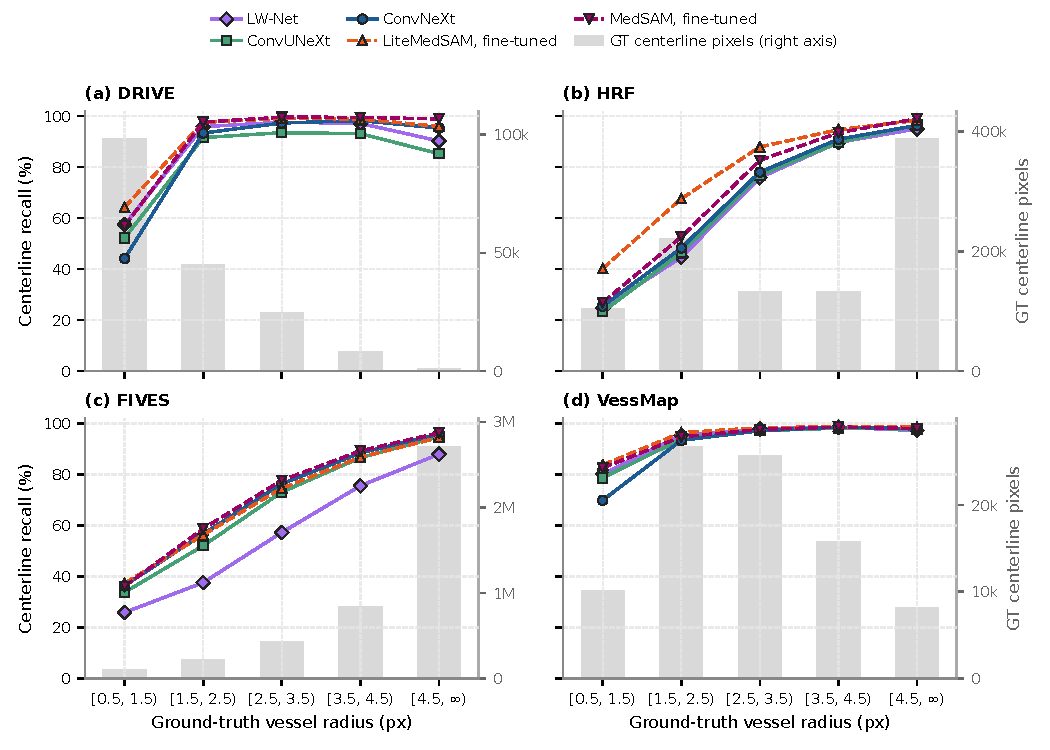
\includegraphics[width=\textwidth]{figures/fig01_recall_by_caliber.pdf}
\caption{Centerline recall by ground-truth vessel radius (means over the test images). The first bin, radius in $[0.5, 1.5)$~px, is $\thinrecall$. Grey bars (right axis, own scale per panel): ground-truth centerline pixels per bin, summed over the test images.}
\label{fig:recall_caliber}
\end{figure*}

A model can raise its $\thinrecall$ by over-segmenting, for example by predicting vessels that are not in the ground truth. Fig.~\ref{fig:thin_pr} therefore plots the centerline precision of thin vessels, $P_{\mathrm{thin}}$, which is computed on the thin centerline pixels of the prediction (Section~\ref{subsec:method_metrics}), so thin vessels that a model draws outside the ground truth lower it.

\begin{figure*}[tbp]
\centering
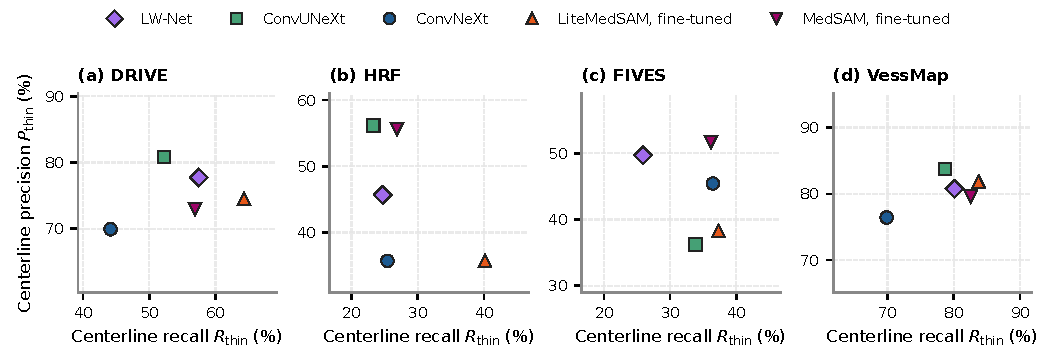
\includegraphics[width=\textwidth]{figures/fig02_thin_precision_recall.pdf}
\caption{Centerline precision against centerline recall of thin vessels, per dataset (means over the test images). Every panel spans the same width on both axes.}
\label{fig:thin_pr}
\end{figure*}

On HRF and FIVES, the $P_{\mathrm{thin}}$ of fine-tuned \medsam{} was not significantly lower than that of any CNN, and on FIVES it was the highest of the five models. On DRIVE and VessMap, it was significantly lower than that of \convunext{}, the best CNN, by 7.8 and 4.2 points, and on DRIVE also than that of \lwnet{}. The higher $\thinrecall$ of \litemedsam{} came with a lower $P_{\mathrm{thin}}$ than that of the best CNN on every dataset, significantly on DRIVE, HRF and FIVES. Table~\ref{tab:pvalues} gives the test of every pair of configurations.

\begin{figure*}[tbp]
\centering
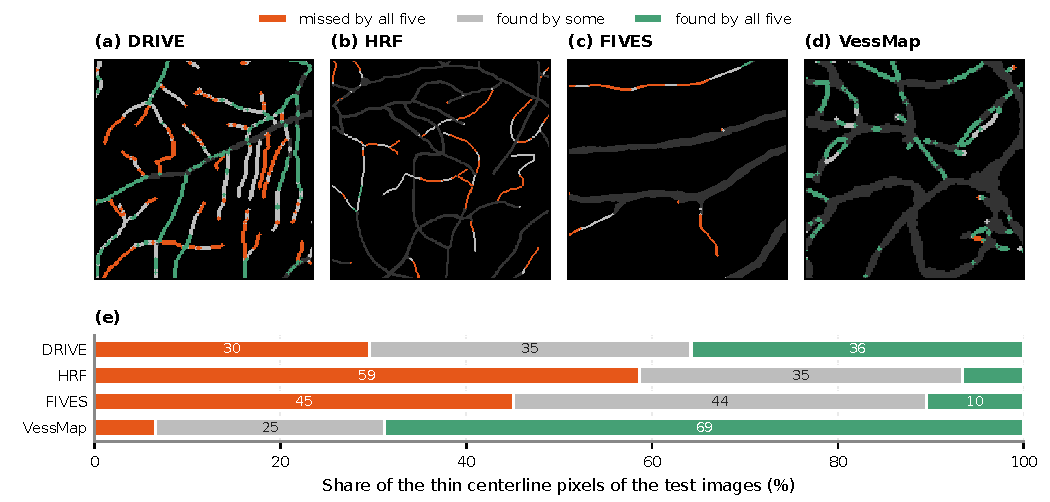
\includegraphics[width=\textwidth]{figures/fig07_thin_errors.pdf}
\caption{Ground-truth thin centerline pixels found by all five models of Table~\ref{tab:global_baseline}, by some or by
none (\medsam{} with the upscaled protocol). (a--d) The window of each test set with the most thin centerline pixels
(160, 320, 256 and 128~px), over the ground-truth vessels (dark grey on black). (e) Shares over all test images.}
\label{fig:thin_errors}
\end{figure*}

Fig.~\ref{fig:thin_errors} shows where the five models find and miss thin vessels. On every dataset, most thin
centerline pixels were found by all five models or missed by all five, so the models succeed and fail largely on the
same thin vessels. A missed thin centerline pixel is either close to a predicted vessel, within 2~px, when the model
drew the vessel slightly offset or narrower, or far from any predicted vessel, when the model did not draw it. On HRF
and FIVES, the largest share was missed by all five and most misses were far; on DRIVE and VessMap, more of the misses
were close, and a metric with a distance tolerance of 2~px would count them as found. The thin vessels that separate the models are a minority of the thin centerline, which
is consistent with the absence of a significant difference in $\thinrecall$ between fine-tuned \medsam{} and the best
CNN.

\subsection{Cost and the compact plain ViT}
\label{subsec:results_cost}

\begin{figure*}[tbp]
\centering
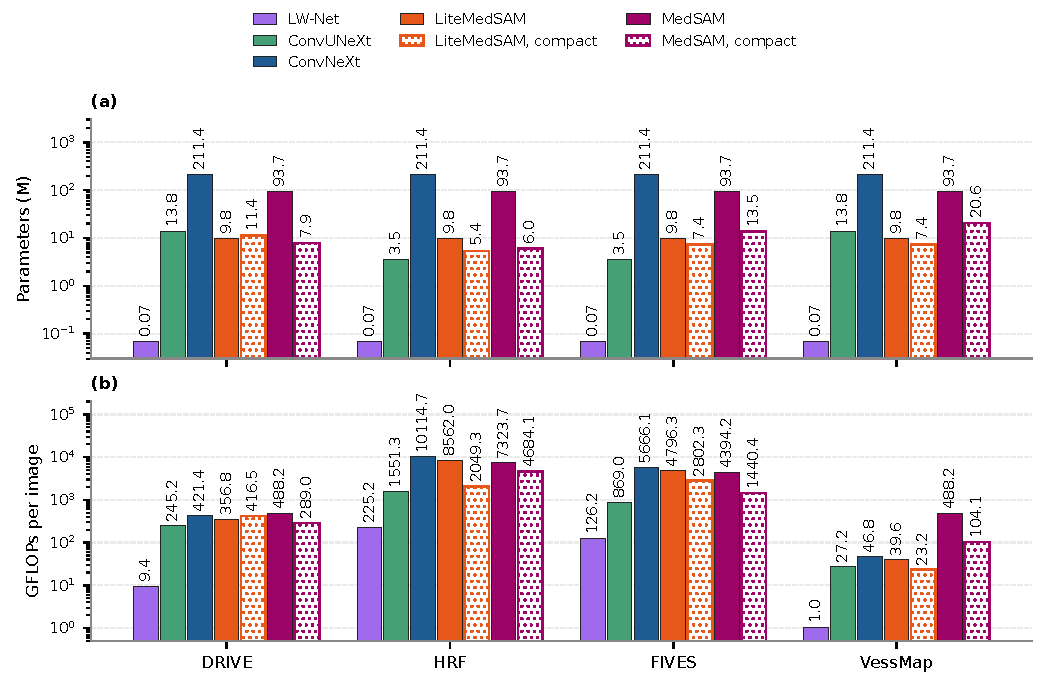
\includegraphics[width=\textwidth]{figures/fig03_cost.pdf}
\caption{Cost of each architecture: (a)~parameters and (b)~GFLOPs per test image, log scale. Fine-tuned and from-scratch runs share one bar.}
\label{fig:cost}
\end{figure*}

\begin{figure*}[tbp]
\centering
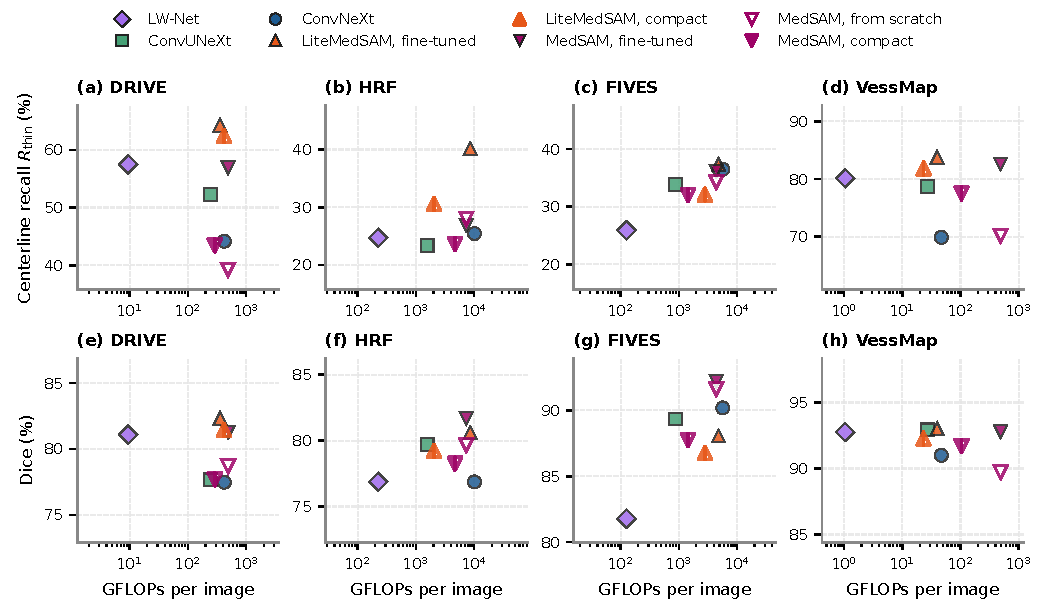
\includegraphics[width=\textwidth]{figures/fig04_compact_tradeoff.pdf}
\caption{$\thinrecall$ (a--d) and Dice (e--h) against GFLOPs per test image (log scale; means over the test images). Compact: \medsam{} and \litemedsam{} with a 256~px window and a searched size, trained from scratch. Within a row, every panel spans the same range width.}
\label{fig:compact_tradeoff}
\end{figure*}

Fig.~\ref{fig:cost} gives the parameters and the GFLOPs per test image of each architecture. \medsam{} had the second-largest parameter count, after \convnext{}, and the highest cost per image on DRIVE and VessMap, whose images are smaller than its 1024~px window and are upscaled to it. On the larger HRF and FIVES images, the models with 256~px windows need many more windows per image than \medsam{}, so \convnext{} and \litemedsam{} cost more per image than \medsam{}. The hybrid \litemedsam{}, in the second class by parameters, had the highest mean $\thinrecall$ on every dataset but a lower $P_{\mathrm{thin}}$ than the best CNN, significantly on three datasets (Section~\ref{subsec:results_thin}), and on HRF and FIVES it cost more per image than \medsam{}.

By parameter count, the models fall into three cost classes (Fig.~\ref{fig:cost}a): \medsam{} and \convnext{}; the compact models, \litemedsam{} and \convunext{}; and \lwnet{}. Models can be compared fairly within a class, unless the aim is the highest accuracy at any cost. The classes hold for parameters, not for GFLOPs per image on HRF and FIVES. The search for compact \litemedsam{}, which was not limited to models smaller than \litemedsam{}, returned models of the same order of size and cost as \litemedsam{}, and on DRIVE a slightly larger one (Table~\ref{tab:compact_models}).

Fine-tuned \medsam{}, whose $\thinrecall$ was not significantly different from that of the best CNN on any dataset, belongs to the most expensive class. Its compact version, in the second class, did not keep this performance (Fig.~\ref{fig:compact_tradeoff}): against the best CNN, its $\thinrecall$ was significantly lower on DRIVE and FIVES, and its $P_{\mathrm{thin}}$ and Dice were significantly lower on all four datasets (Table~\ref{tab:pvalues}). Its cost per image was within the range of the CNNs except on VessMap. Compact \medsam{} differs from fine-tuned \medsam{} in size, initialization, patch size, input window and, on DRIVE and VessMap, input scale, so this comparison does not separate them; Fig.~\ref{fig:pretraining} compares the same architectures with and without pre-training.

The search for compact \medsam{} selected finer patches than the 16~px of \medsam{}: 4~px, and 8~px on FIVES (Table~\ref{tab:patch_size}). With 16~px patches, its best validation Dice was 15.7\% on DRIVE and 14.0\% on HRF. Other hyperparameters varied between these trials, so Table~\ref{tab:patch_size} is not a controlled comparison of patch sizes.

\subsection{Pre-training and training difficulty}
\label{subsec:results_pretraining}

\begin{figure*}[tbp]
\centering
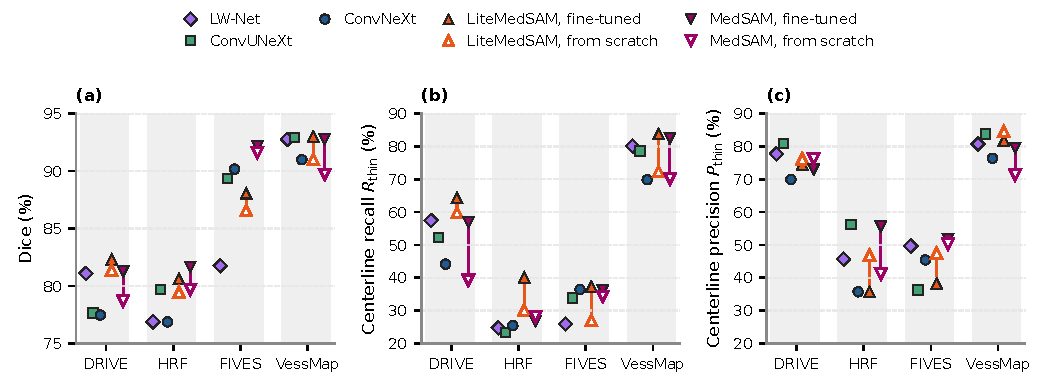
\includegraphics[width=\textwidth]{figures/fig05_pretraining.pdf}
\caption{Effect of pre-training: (a)~Dice, (b)~$\thinrecall$ and (c)~$P_{\mathrm{thin}}$ of the two transformer-based models fine-tuned (filled) and trained from scratch (hollow), next to the CNNs (means over the test images). Panels (b) and (c) share one vertical range.}
\label{fig:pretraining}
\end{figure*}

Fig.~\ref{fig:pretraining} compares \medsam{} and \litemedsam{} fine-tuned from their pre-trained weights with the same architectures trained from scratch, next to the three CNNs; Table~\ref{tab:pretraining_gain} in Appendix~\ref{app:results_detail} gives the gain from pre-training, fine-tuned minus from scratch.

\begin{figure*}[tbp]
\centering
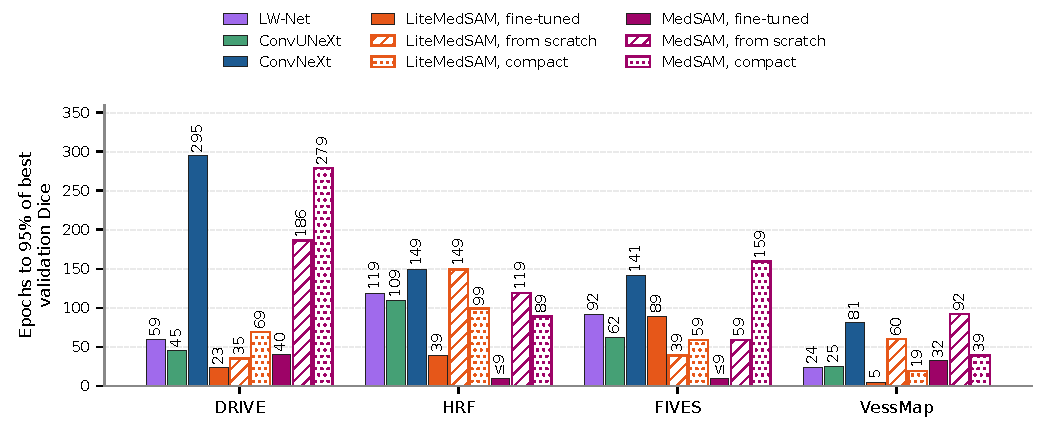
\includegraphics[width=\textwidth]{figures/fig06_convergence.pdf}
\caption{Epochs until the selected run first reached 95\% of its best validation Dice (validation every epoch or every 10 epochs; ``$\le$'': reached at the first validation). One run per configuration.}
\label{fig:convergence}
\end{figure*}

Pre-training raised the Dice of \medsam{} significantly on every dataset (Fig.~\ref{fig:pretraining}a; Table~\ref{tab:pretraining_gain}). Its effect on the $\thinrecall$ of \medsam{} depended on the dataset: it rose by 17.6 and 12.4 points on DRIVE and VessMap, much less on FIVES and not significantly on HRF. For the hybrid \litemedsam{}, pre-training raised $\thinrecall$ significantly on every dataset and Dice by less. Trained from scratch, \litemedsam{} had a higher $P_{\mathrm{thin}}$, significantly on HRF and FIVES. Without pre-training, the $\thinrecall$ of \medsam{} was significantly lower than that of the best CNN on DRIVE, FIVES and VessMap, and not on HRF.

Without pre-training, \medsam{} also needed more epochs to reach 95\% of its best validation Dice on every dataset (Fig.~\ref{fig:convergence}), and so did compact \medsam{}. For \litemedsam{} the pattern was mixed: from scratch it needed more epochs on DRIVE, HRF and VessMap and fewer on FIVES. Each of these values comes from one training run.

Table~\ref{tab:medsam_vs_cnn} compares fine-tuned \medsam{} with the best CNN of each metric and dataset. On HRF and FIVES, its Dice was significantly higher, by 2.0 points, with no significant difference in either thin-vessel metric (Tables~\ref{tab:medsam_vs_cnn} and~\ref{tab:pvalues}); on DRIVE and VessMap, its Dice was not significantly different. It also reached 95\% of its best validation Dice in fewer epochs than the CNN with the highest Dice on DRIVE, HRF and FIVES.

For \medsam{}, the Dice gain from pre-training was smallest on FIVES, the dataset with the most training images, with no order by number of images among the other three. For \litemedsam{}, the gains in Dice and $\thinrecall$ instead grew from DRIVE to HRF to VessMap, in the order of their number of training images, and were not smallest on FIVES (Table~\ref{tab:pretraining_gain}). The four datasets also differ in resolution, imaging domain and the upscaling of \medsam{}, so the number of training images is not isolated.

% Generated by paper/figures_tables/tab03_medsam_vs_cnn.py -- do not edit by hand.
% Source: results/per_image_metrics.csv (MedSAM DRIVE/VessMap upscaled protocol); results/convergence.csv.
\begin{table*}[tbp]
\caption{Fine-tuned \medsam{} against the best CNN of each metric and dataset (L: \lwnet{}, U: \convunext{}, N:
\convnext{}); $\Delta$: \medsam{} minus the best CNN. Bold: best; $^{*}$: significant. Epochs: of \medsam{} and of the
CNN with the highest Dice
(bold: fewer; ``$\le$'': reached at the first validation).}
\label{tab:medsam_vs_cnn}
\begin{ruledtabular}
\begin{tabular}{lcccccccc}
 & \multicolumn{3}{c}{Dice} & \multicolumn{3}{c}{$\thinrecall$} & \multicolumn{2}{c}{Epochs} \\
\cmidrule(lr){2-4} \cmidrule(lr){5-7} \cmidrule(lr){8-9}
Dataset & \medsam{} & Best CNN & $\Delta$ & \medsam{} & Best CNN & $\Delta$ & \medsam{} & CNN \\
\midrule
\shortstack{DRIVE\\($n=20$)} & {\boldmath$81.3 \pm 1.3$} & $81.1 \pm 2.4$\textsuperscript{L} & $+0.2$ & $56.9 \pm 11.8$ & {\boldmath$57.5 \pm 12.1$}\textsuperscript{L} & $-0.6$ & \textbf{40} & 59 \\
\shortstack{HRF\\($n=14$)} & {\boldmath$81.7 \pm 4.5$} & $79.7 \pm 5.1$\textsuperscript{U} & $+2.0^{*}$ & {\boldmath$26.9 \pm 17.2$} & $25.4 \pm 13.5$\textsuperscript{N} & $+1.5$ & \textbf{$\le$9} & 109 \\
\shortstack{FIVES\\($n=200$)} & {\boldmath$92.2 \pm 8.5$} & $90.2 \pm 8.5$\textsuperscript{N} & $+2.0^{*}$ & $36.2 \pm 11.9$ & {\boldmath$36.5 \pm 12.2$}\textsuperscript{N} & $-0.3$ & \textbf{$\le$9} & 141 \\
\shortstack{VessMap\\($n=30$)} & $92.8 \pm 2.1$ & {\boldmath$92.9 \pm 2.1$}\textsuperscript{U} & $-0.1$ & {\boldmath$82.6 \pm 14.1$} & $80.1 \pm 12.2$\textsuperscript{L} & $+2.5$ & 32 & \textbf{25} \\
\end{tabular}
\end{ruledtabular}
\end{table*}


% Generated by paper/figures_tables/tab02_padding_protocol.py -- do not edit by hand.
% Source: results/per_image_metrics.csv (native = padded and upscaled protocols); GFLOPs per window from
% results/cost.csv; windows per image from MONAI's grid.
\begin{table*}[tbp]
\caption{The same \medsam{} checkpoints evaluated with the padded and the upscaled protocol; $\Delta$: upscaled minus
padded. Bold: best; $^{*}$: significant. $P_{\mathrm{thin}}$, VessMap, from scratch, padded: mean over 29 images (one image without predicted thin vessels).}
\label{tab:padding}
\begin{ruledtabular}
\begin{tabular}{llcccccc}
 & & \multicolumn{3}{c}{DRIVE ($n=20$)} & \multicolumn{3}{c}{VessMap ($n=30$)} \\
\cmidrule(lr){3-5} \cmidrule(lr){6-8}
\medsam{} & Metric & Padded & Upscaled & $\Delta$ & Padded & Upscaled & $\Delta$ \\
\midrule
\multirow{3}{*}{Fine-tuned} & Dice & $75.2 \pm 1.8$ & {\boldmath$81.3 \pm 1.3$} & $+6.1^{*}$ & $78.7 \pm 7.5$ & {\boldmath$92.8 \pm 2.1$} & $+14.1^{*}$ \\
 & $\thinrecall$ & $39.0 \pm 10.9$ & {\boldmath$56.9 \pm 11.8$} & $+17.9^{*}$ & $41.3 \pm 12.7$ & {\boldmath$82.6 \pm 14.1$} & $+41.3^{*}$ \\
 & $P_{\mathrm{thin}}$ & $58.8 \pm 7.9$ & {\boldmath$73.0 \pm 6.1$} & $+14.2^{*}$ & $76.8 \pm 13.2$ & {\boldmath$79.6 \pm 14.8$} & $+2.8$ \\
\midrule
\multirow{3}{*}{From scratch} & Dice & $65.7 \pm 3.0$ & {\boldmath$78.7 \pm 1.6$} & $+13.0^{*}$ & $68.2 \pm 6.4$ & {\boldmath$89.7 \pm 3.7$} & $+21.5^{*}$ \\
 & $\thinrecall$ & $25.3 \pm 8.0$ & {\boldmath$39.3 \pm 11.2$} & $+14.0^{*}$ & $43.6 \pm 19.2$ & {\boldmath$70.2 \pm 20.9$} & $+26.6^{*}$ \\
 & $P_{\mathrm{thin}}$ & $56.5 \pm 8.8$ & {\boldmath$76.2 \pm 7.0$} & $+19.7^{*}$ & $57.5 \pm 21.3$ & {\boldmath$71.4 \pm 14.1$} & $+13.9^{*}$ \\
\end{tabular}
\end{ruledtabular}
\end{table*}


\subsection{Inference protocol of MedSAM: padding versus upscaling}
\label{subsec:results_padding}

On DRIVE and VessMap, both protocols of Section~\ref{subsec:method_metrics} run one 1024~px window per image and have the same cost. The comparison is therefore not about a cheaper way to run \medsam{}: with the same checkpoints, padding makes each vessel span fewer input pixels than upscaling does.

The padded protocol gave a significantly lower Dice and $\thinrecall$ than the upscaled protocol for fine-tuned \medsam{} and \medsam{} trained from scratch on both datasets (Table~\ref{tab:padding}). For fine-tuned \medsam{}, $\thinrecall$ fell by 17.9 points on DRIVE and 41.3 points on VessMap, below the range of the CNNs on both datasets.

\subsection{Discussion}
\label{subsec:discussion}

The thin-vessel results of fine-tuned \medsam{} (Section~\ref{subsec:results_thin}) do not support the expectation that a plain ViT misses thin vessels, at least for \medsam{}, pre-trained on medical images~\cite{ma2024segment}, evaluated with the upscaled protocol.

The results bear on the argument that a 16~px token dilutes thin vessels (Section~\ref{sec:related_work}) in two ways, neither of which isolates it. On DRIVE and VessMap, \medsam{} saw the images upscaled, so a 16~px patch covered a square of about 9 and 4 native pixels on a side (Section~\ref{subsec:method_training}). With the native image padded into the window, the same checkpoints lost much of their $\thinrecall$ (Table~\ref{tab:padding}). This is consistent with the extent of a token in native pixels mattering for thin vessels, but padding also changes the scale at which the model sees the image relative to training, and the two explanations cannot be separated here. On HRF and FIVES, where \medsam{} tokenized native pixels in 16~px patches, its $\thinrecall$ was also within or above the range of the CNNs, although $\thinrecall$ was low for every model on these two datasets.

The hybrid \litemedsam{} had the highest mean $\thinrecall$ on every dataset but a lower $P_{\mathrm{thin}}$ than the best CNN on all four, so its higher recall is not by itself evidence of a better segmentation of thin vessels.

Our results on the compact plain ViT are limited in two ways. First, compact \medsam{} differs from fine-tuned \medsam{} in several properties at once (Section~\ref{subsec:results_cost}), so the results cannot say which of these accounts for its loss of thin-vessel performance; they show only that the plain ViT obtained its $\thinrecall$ as a model of the most expensive class and that a compact version in the second class did not keep it (Section~\ref{subsec:results_cost}). Second, the search selected one architecture per dataset by validation Dice and was not designed to study model size or patch size. Its preference for 4 or 8~px patches over 16~px patches on every dataset is therefore only consistent with the argument that a 16~px token dilutes thin vessels, for a plain ViT trained from scratch on a 256~px window. A study that varies the size of the plain ViT in a controlled way, including compact versions smaller than those selected here, could show where its thin-vessel performance is lost.

Our finding on thin vessels holds for the pre-trained \medsam{} only: trained from scratch, it fell below the best CNN in $\thinrecall$ on three datasets (Section~\ref{subsec:results_pretraining}). This gain from pre-training is measured against our from-scratch recipe, which used the learning rates searched for fine-tuning, batch sizes of 1 to 4 and no warm-up; a recipe designed for training a ViT from scratch could reduce it. Trained from scratch, the hybrid detected fewer thin vessels on every dataset and, on HRF and FIVES, a larger share of the thin vessels it drew was in the ground truth, which is consistent with a more conservative segmentation of thin vessels.

Our data answer only in part how the gain from pre-training depends on the number of training images, and the answer differs between the two models. For \medsam{}, the Dice gain was smallest on FIVES, the dataset with the most training images, which is consistent with pre-training adding less when more training images are available; its $\thinrecall$ gain was large on the two datasets it saw upscaled and small or absent on the other two, an order that does not follow the number of training images. For \litemedsam{}, the gains grew with the number of training images over the three smaller datasets and were not smallest on FIVES, which does not fit that reading. With four datasets that also differ in resolution, domain and upscaling, these are orders over four points, not estimates of how the gain depends on the number of images.

The advantage of the pre-trained plain ViT over the CNNs trained from scratch was small: a higher Dice on HRF and FIVES without a significant difference in either thin-vessel metric, and none on DRIVE and VessMap, where its $P_{\mathrm{thin}}$ was significantly lower than that of the best CNN.

We did not measure how finely each dataset was annotated, a possible factor in the thin-vessel results. Thin vessels hold a much larger share of the ground-truth centerline on DRIVE than on FIVES (Section~\ref{subsec:results_overall}). Part of this difference comes from resolution, since a vessel of a given width spans more pixels in the larger HRF and FIVES images. Part may come from annotation detail, if DRIVE was annotated down to finer vessels than FIVES, a dataset with many more images. A thin vessel that a model detects but the annotation omits lowers its $P_{\mathrm{thin}}$, which may contribute to the lower $P_{\mathrm{thin}}$ of every model on HRF and FIVES than on DRIVE and VessMap (Fig.~\ref{fig:thin_pr}).

We observed the effect of padding for one model on two datasets, but it is a methodological point for evaluating a plain ViT on images smaller than its input window: on DRIVE and VessMap, whether fine-tuned \medsam{} had a $\thinrecall$ within the range of the CNNs depended on the inference protocol (Table~\ref{tab:padding}). A study that evaluates such a model on small images should therefore evaluate it at the scale used in training and state that scale.

Six limitations concern how the models were trained, selected and measured. Each configuration was trained once, with one random seed, so the variation between training runs is unknown. For Little W-Net, the published 95\% confidence interval of the mean DRIVE Dice over five runs is $\pm 0.11$ points~\cite{galdran2020littlewnetcouldstateoftheart}, but ours was not measured. The Wilcoxon tests take the test images as the sample, so they generalize over test images, not over training runs; on HRF, with 14 test images, they detect only large or very consistent differences. On HRF, FIVES and VessMap, checkpoint selection, early stopping and the hyperparameter search used the test images (Section~\ref{subsec:method_problem_data}). The comparison across architectures pairs CNNs trained from scratch with fine-tuned transformer-based models, so it mixes architecture and initialization: ImageNet weights exist for the ConvNeXt-Large encoder~\cite{liu2022convnet}, but they come from natural images, so we did not use them, and we found no public CNN pre-trained on a medical image collection comparable to that of \medsam{}. \medsam{} saw DRIVE and VessMap upscaled, and on every dataset its window covered 16 times the area of the other models' windows; the CNNs were not trained at this scale or window, so the comparison does not separate the architecture from the input scale and window. Finally, we measured cost as parameters and GFLOPs, not as latency or throughput.
